% Chapter Template

\chapter{Background}

\label{Chapter1} 

\begin{comment}
-------------------------------------------------
%								Chapter layout
2. Background
	a. Leap Motion (v2)
		i. Java API
		ii. Native Libraries
		iii. Limitations of Sensor and Documentation
	b. JavaFx
		i. Java vs FXML
		ii. SceneBuilder
		iii. Jfoenix
		iv. ControlsFx
	c. IntelliJ IDE
		i. Unix Style Terminal on Windows
-------------------------------------------------
\end{comment}



%------------------------------------------------
%	SECTION 1 Leap Motion (v2)
%------------------------------------------------

\section{Leap Motion (v2)}
--introduction to the sensor. when it was made. company behind it. what its used for. price



%----------------------------------- Leap Motion Java API
\subsection{Java API}
hand class, fingers bones. vector. 



%----------------------------------- Native Libraries
\subsection{Native Libraries}
--read the page on lm website and summarize




%----------------------------------- Limitations of Sensor and Documentation
\subsection{Limitations of Sensor and Documentation}
--occulusion
--discontinuation of publishing v2 apps
--sensor resetting by opening palm
--not enough documentation for linux/ubuntu. 




%------------------------------------------------
%	SECTION 2 JavaFX
%------------------------------------------------

\section{JavaFx}

JavaFX is a framework provided by Oracle Corporation that is intended to replace the Swing framework as the standard GUI library for developing desktop applications that can be run on any platform that supports Java. Since the JavaFX 2.0 release, JavaFX application can be written in pure Java code. Before that release, applications written using JavaFX libraries had to be written in Java FX Script, a scripting language designed and used specifically for the purpose of creating GUI applications with JavaFX. This project uses the latest version of this framework, JavaFX 8, which also added support for 3D graphics and sensor support. 


%----------------------------------- Java vs FXML
\subsection{Java vs FXML}

When writing a JavaFX application, there are two very different approaches that can be used to create the actual user interface (UI) for the application. These are pure Java code and FXML. A brief introduction both of these approaches will be given below. 

The pure Java approach constructs the JavaFX application scene graph procedurally through code. Below is a simple “Hello World” program that shows a quick example of this approach in action.

\begin{figure}[th]
\centering
\begin{lstlisting}
public class HelloWorld extends Application {
public static void main(String[] args) {
	launch(args);
}

@Override
public void start(Stage primaryStage) {
	primaryStage.setTitle("Hello World!");
	Button btn = new Button();
	btn.setText("Say 'Hello World'");
	btn.setOnAction(new EventHandler<ActionEvent>() {
		@Override
		public void handle(ActionEvent event) {
			System.out.println("Hello World!");
		}
	});
	
	StackPane root = new StackPane();
	root.getChildren().add(btn);
	primaryStage.setScene(new Scene(root, 300, 250));
	primaryStage.show();
}
}
\end{lstlisting}
\caption{A simple hello world program using JavaFX written using just Java code.}
\label{fig:helloWorldJavaFX1}
\end{figure}

This small snippet of code contains the overall structure and all of the basic components of a JavaFX application. The first point to note is that the main class which will run the JavaFX application must extend from the abstract base class called javafx.application.Application and implement is abstract start() method. The start() method serves as the main entry point for all JavaFX applications. In the application’s main() method, which is common to all Java applications, a call must be made to the launch() method which is a method defined in the base Application JavaFX class that actually launches the application in doing so makes a call to the start() method. 

The start() method receives a parameter of type Stage which serves as the primary Stage object for the application. Stage is the top-level user interface container object used by JavaFX to house the whole application. In colloquial terms it can be considered to be the “window” object of the whole application. The Stage object is has a setScene() method which requires a Scene object to be passed in. Scene class is the container of current content being displayed by the application. An application can have multiple scenes which display different pages of the the application. In JavaFX, the actual UI components, such as the StackPane layout Node shown in the simple HelloWorld example above, must be added to the Scene object in order for them to be displayed. This relationship between the Stage, Scene and “root” Node components of a JavaFX application is depicted in Figure \ref{fig:stageSceneRoot}.
\begin{figure}[th]
\centering
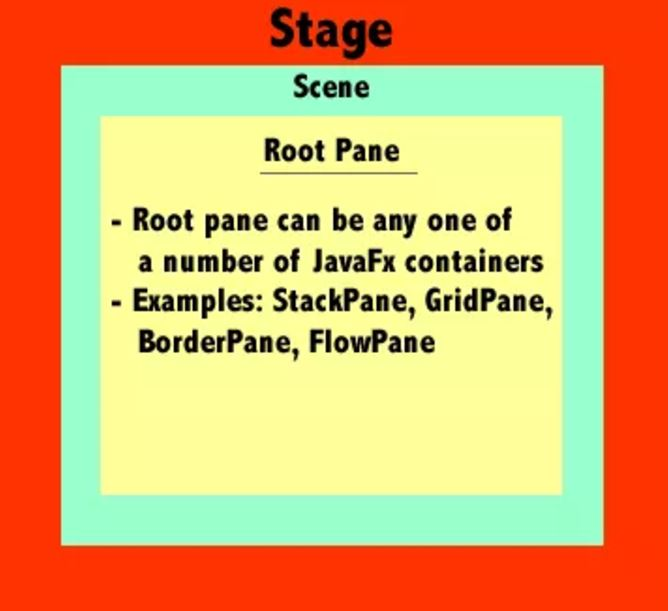
\includegraphics[scale=0.5]{Figures/stageSceneRoot.JPG}
\caption{The layout components of every JavaFX application.}
\label{fig:stageSceneRoot}
\end{figure}


The UI components all extend from a parent Node class. One of the improvements that JavaFX brought in regards to its predecessor Swing, is that it represents the entire content of the scene as a tree. More specifically, all of the nodes displayed in a Scene container object must extend from a root level node and be part of the hierarchical scene graph of nodes. Figure \ref{fig:javafxSceneGraph}  displays an example of the JavaFX scene graph. 
\begin{figure}[th]
\centering
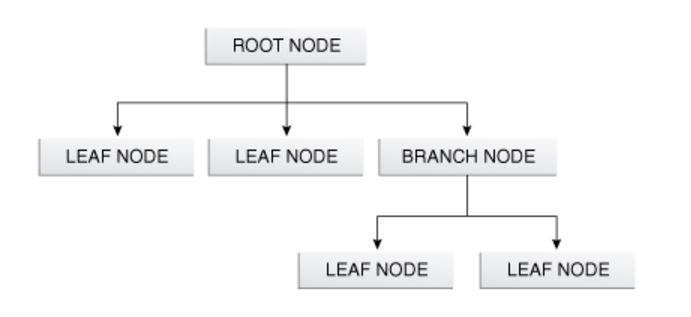
\includegraphics[scale=0.5]{Figures/javafx_scenegraph.JPG}
\caption{The Scene Graph architectural model for UI components in JavaFX applications.}
\label{fig:javafxSceneGraph}
\end{figure}


Now that the pure Java code approach of writing JavaFX applications has been introduced, let us discuss the other approach to writing JavaFX applications; FXML. FXML is a XML-based language created by Oracle Corporation for the purpose of making it easier to define the UI of a JavaFX application. While the pure Java code approach is a much more imperetive and procedural way to write JavFX applications, FXML is a more declartive way. It resembles HTML and can also reference a controller java class which can access and modify the UI elements defined in the FXML file. Figure \ref{fig:simpleFXML} shows a very simple FXML file that creates a VBox layout and adds a button to it. This FXML file also has a Java controller class attached to it which is called MyController.java and shown in Figure \ref{fig:simpleController}

\begin{figure}[th]
\centering
\begin{lstlisting}
<?xml version="1.0" encoding="UTF-8"?>
<?language JavaScript?>
<?import javafx.scene.control.*?>
<?import javafx.scene.layout.*?>

<VBox fx:id="myView" layoutX="10.0" layoutY="10.0" xmlns:fx="http://javafx.com/fxml/1" xmlns="http://javafx.com/javafx/2.2" fx:controller="MyController">
  <children>
    <Button fx:id="okBtn" alignment="CENTER_RIGHT" contentDisplay="CENTER" mnemonicParsing="false" onAction="#printHelloWorld" text="OK" textAlignment="CENTER" />
  </children>
</VBox>
\end{lstlisting}
\caption{A FXML file defining a simple layout and referencing a controller java class.}
\label{fig:simpleFXML}
\end{figure}


\begin{figure}[th]
\centering
\begin{lstlisting}
public class MyController 
{
	@FXML
	private void initialize() 
	{
	// this method runs first after all the UI components have been loaded and bound.
	}
	
	@FXML
	private void printHelloWorld() 
	{
		System.out.println("hello world!");
	}
}
\end{lstlisting}
\caption{A controller for the FXML file. The "FXML" annotation in is used to bind certain elements to java objects in the class.}
\label{fig:simpleController}
\end{figure}






(ending paragraph discussion)
The large difference between these two different approaches makes it difficult to combine them effectively, but it is possible to use them in conjunction with each other (as this project does in the design of its application). 









%----------------------------------- SceneBuilder
\subsection{SceneBuilder}
--explain what scenbuilder is. mention gluon. how
--how to use it. 
-- show different windows and what they mean. 